\section{Lezione 10 - 06/10/2023}
\subsection{Alberi Perfettamente Bilanciati}
Gli alberi perfettamente bilanciati sono particolare tipi di albero binario in cui vale la seguente condizione:
$$ | |T->sx| - |T->dx| |  \le 1 $$ 
La cardinalità (numeri di elementi) del sottoalbero sinistro deve differire di \textbf{al più 1} elemento del sottoalbero destro.\\
Non tutti gli alberi completi sono perfettamente bilanciati ma tutti gli alberi perfettamente bilanciati sono pieni.

\begin{figure}[H]
    \centering
    \begin{subfigure}[b]{0.45\textwidth}
        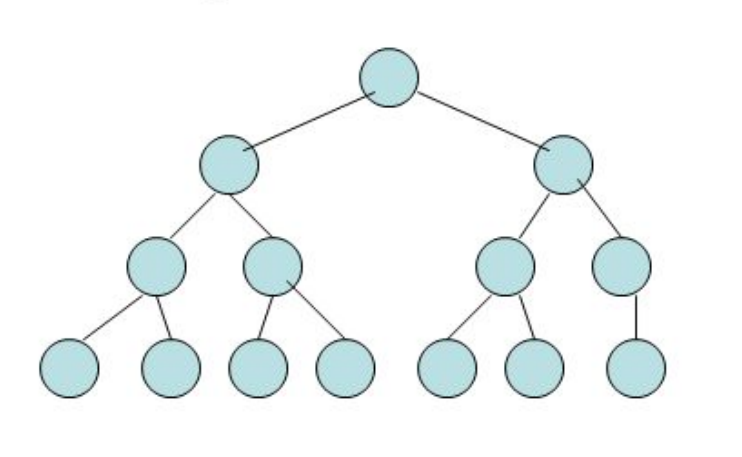
\includegraphics[width=\textwidth]{APB} 
        \caption{È un APB}
    \end{subfigure}
    \hfill
    \begin{subfigure}[b]{0.45\textwidth}
        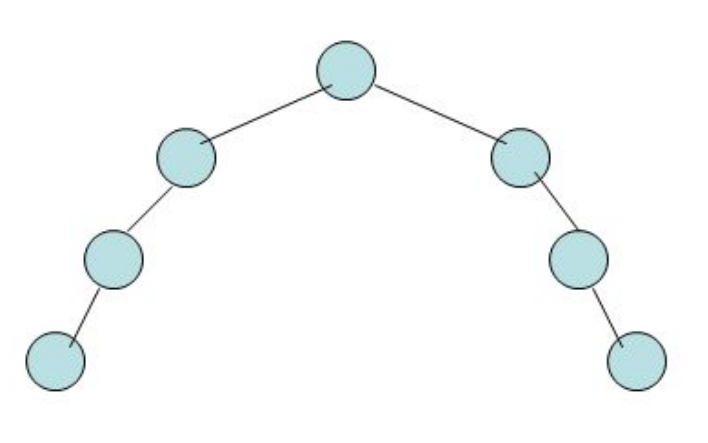
\includegraphics[width=\textwidth]{NAPB} 
        \caption{NON è un APB}
    \end{subfigure}
    %\caption{Didascalia generale per entrambe le immagini}
\end{figure}


\subsection{Alberi AVL}
Gli alberi AVL sono particolare tipi di albero binario in cui vale la seguente condizione:
$$ | h(T->sx) - h(|T->dx) |  \le 1 $$ 
Quindi l'altezza del sottoalbero sinistro di T e quella del sottoalbero destro di T differiscono al più di uno, ovviamente si applica ad ogni sottonodo.\\
A differenza degli alberi perfettamente bilanciati, non si pone un limite sulla cardinalità dell'insieme ma bensi sull'\textbf{altezza} dei sottoalberi.\\

\begin{figure}[H]
    \centering
    \begin{subfigure}[b]{0.45\textwidth}
        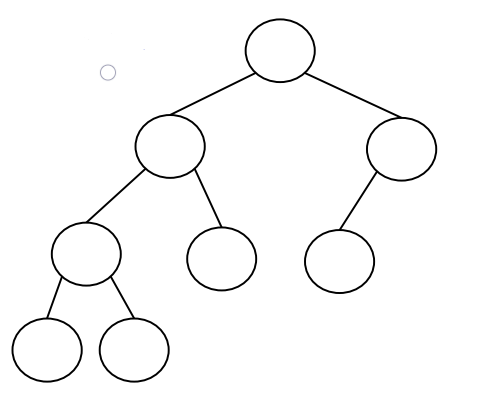
\includegraphics[width=\textwidth]{AVL} 
        \caption{È un AVL}
    \end{subfigure}
    \hfill
    \begin{subfigure}[b]{0.45\textwidth}
        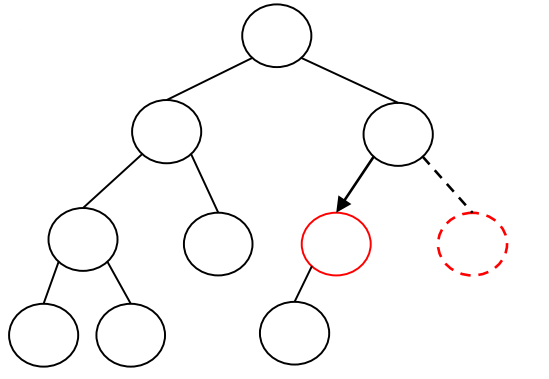
\includegraphics[width=\textwidth]{NAVL} 
        \caption{NON è un AVL}
    \end{subfigure}
    %\caption{Didascalia generale per entrambe le immagini}
\end{figure}
\begin{center}
    \textbf{Un albero pieno è sia ABL che AVL}    
\end{center}

\subsection{Alberi AVL Minimi}
Fissato $h$, l'albero AVL minimo di altezza $h$ è l'albero AVL di altezza $h$ col minor numero di nodi possibile.\\
Per ogni altezza andiamo a mostrare un possibile albero:

\begin{figure}[H]
    \centering
    \begin{subfigure}[b]{0.35\textwidth}
        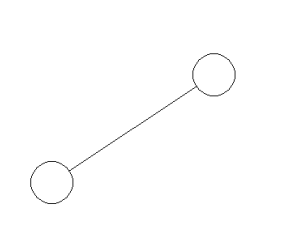
\includegraphics[width=\textwidth]{AVLh1} 
        \caption{AVL minimo di altezza 1}
    \end{subfigure}
    \hfill
    \begin{subfigure}[b]{0.45\textwidth}
        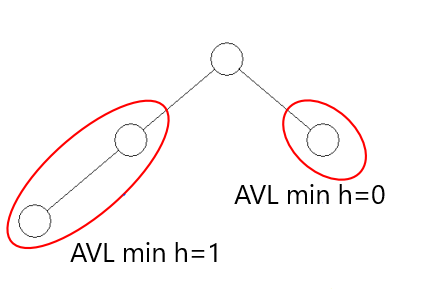
\includegraphics[width=\textwidth]{AVLh2} 
        \caption{AVL minimo di altezza 2}
    \end{subfigure}
    \hfill
    \begin{subfigure}[b]{0.45\textwidth}
        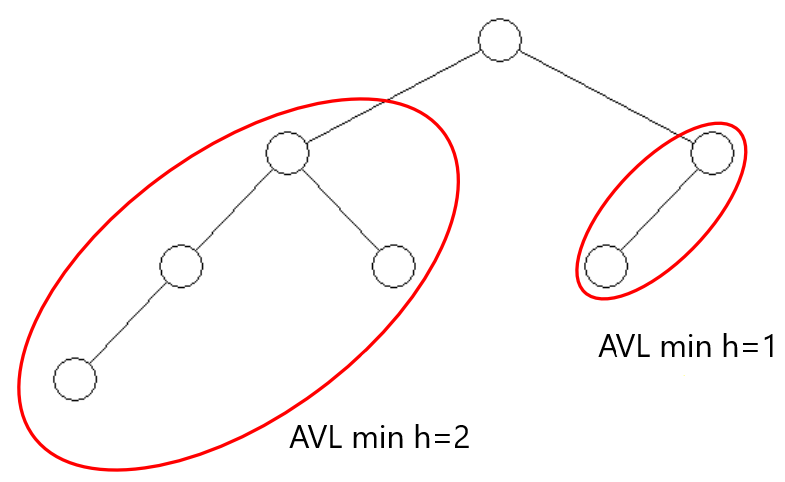
\includegraphics[width=\textwidth]{AVLh3} 
        \caption{AVL minimo di altezza 3}
    \end{subfigure}
    \hfill
    \begin{subfigure}[b]{0.45\textwidth}
        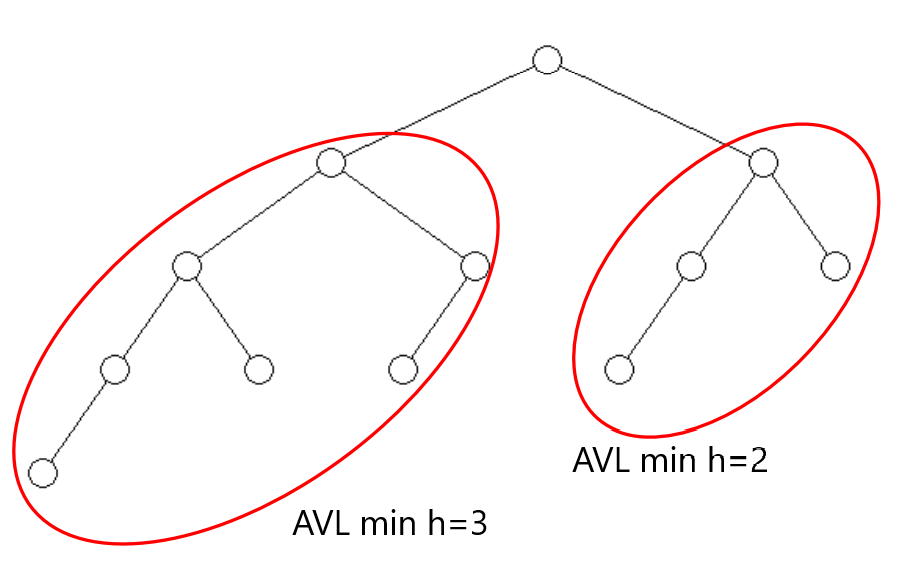
\includegraphics[width=\textwidth]{AVLh4} 
        \caption{AVL minimo di altezza 4}
    \end{subfigure}
\end{figure}
Possiamo notare un certo pattern che si ripeto, nello specifico dato un albero di altezza $h$ il sottoalbero sinistro sarà $h-1$ e il ciaosottoalbero destro $h-2$.\\
Andiamo a generalizzare questa osservazione:
$$ N(h)= \begin{cases}
    h+1 & \text{se } h=0,1\\
    1+N(h-1)+N(h-2) & \text{e poniamo per assurse } h \ge 2
\end{cases} $$
\textbf{DIM $h \ge 2$:}\\
Prediamo un generico AVL $T$ minimo, e poniamo per assurdo che il suo sottoalbero sinistro \textbf{è un AVL non minimo}, dunque esisterà un albero $T^{\prime}$ con sottoalbero sinistro che sarà \textbf{AVL minimo}. Quindi è un assurdo il fatto che esisterà un sottoalbero di $T^{\prime}$ di altezza $h-1$ con un numero minore di nodi rispetto al sottoalbero di $T$. In generale dunque se andiamo a dire che $T$ è un Albero AVL minimo, non è possibile che esiste un $T^{\prime}$ con un numero di nodi \textbf{minore} di un albero AVL minore.

Data la formula precendete facciamo una considerazione:\\
\begin{center}
    \begin{tabular}{|c|c|c|c|c|c|c|c|c|c|} % Sostituisci 'c' con 'l' se vuoi l'allineamento a sinistra
        \hline
        Altezza & 0 & 1 & 2 & 3 & 4 & 5 & 6 & 7 & 8 \\
        \hline
        Numeri Nodi & 1 & 2 & 4 & 7 & 12 & 20 & 33 & 54 & 88 \\
        \hline
        Fibonacci & 0 & 1 & 1 & 2 & 3 & 5 & 8 & 13 & 21 \\
        \hline
    \end{tabular}
\end{center}

Possiamo notare come ci siamo un certo collegamento tra i numeri di nodi e la sequenza di fibonacci, nello specifico notiamo come:
$$ N(h) = F(h+3)-1$$
Facciamo un ragionamento su come ricaverci l'altezza dato  la formula chiusa di Fibonacci:
$$ F(x)= \frac{1}{\sqrt{5}} [(\frac{1+\sqrt{5}}{2})^x - \cancel{(\frac{1-\sqrt{5}}{2})^x}]  $$
Andiamo a rimuovere la seconda parte poiché tende a zero.\\
$$ F(x)=c \cdot k^x $$
$$ N(h) = F(h+3)-1 $$
$$ N(h) = c \cdot k^{h+3}-1$$
$$ \frac{N(h)-1}{c} = k^{h+3} $$ 
$$ h =  \log_k (\frac{N(h)-1}{c}) -3 $$
Abbiamo dimostrato che l'altezza è logaritmica sul numero di nodi.\\
Adesso andiamo a dimostrare che la formula dei nodi vale per ogni $h$\\
\textbf{DIM:}
\begin{itemize}
    \item \textbf{Caso base:} $N(0) = F(0+3) - 1 = 1$
    \item \textbf{Caso induttivo:}
    \[
    N(h) = 1 + N(h-1) + N(h-2)
    \]
    Per ipotesi:
    \[
    N(h-1) = F(h+2) - 1
    \]
    \[
    N(h-2) = F(h+1) - 1
    \]
    Quindi:
    \[
    1 + (F(h+2) - 1) + (F(h+1) - 1) = F(h+3) - 1
    \]
\end{itemize}
